\lstset{basicstyle=\footnotesize\sffamily,frame=single}

L'analyse des mod\`eles et outils existants
permettant de d\'efinir et r\'ealiser des architectures de
composants nous a permis d'une part de d\'egager les concepts
fondamentaux relatifs \`a ce domaine : composants, interfaces, ports
et connexions. D'autre part, nous avons constat\'e qu'il existait une certaine distance entre des mod\`eles
permettant de \emph{concevoir} et v\'erifier des propri\'et\'es sur
des architectures de composants, sch\'ematiquement les \emph{langages de
description d'architecture} formels, et d'autre part les plateformes
et implantations concr\`etes permettant de construire et ex\'ecuter
des syst\`emes de composants. Notre objectif est d'\^etre capable
non seulement de raisonner sur des mod\`eles mais aussi d'utiliser
ces sp\'ecifications pour \emph{v\'erifier} des implantations
concr\`etes de mod\`eles, en particulier par le test. Par ailleurs, on souhaite que ces
mod\`eles soient suffisamment abstraits de l'implantation pour \^etre
\emph{r\'eutilisables}, ce dans l'optique de construire une
d\'emarche formalis\'ee d'\emph{ing\'enierie dirig\'ee par les
mod\`eles}. Le but final est bien entendu de d\'ecoupler la
mod\'elisation des processus m\'etiers de la conception des
syst\`emes les r\'ealisant.

Dans ce chapitre, nous pr\'esentons en d\'etail mais de mani\`ere
informelle un \emph{mod\`ele de
composants abstraits} nomm\'e \textsf{FIDL} pour \emph{Formal Interface
Definition Language}. La premi\`ere partie de ce chapitre est 
une exposition informelle des principaux \'el\'ements de ce
mod\`ele qui reprend les concepts
fondamentaux d\'egag\'es au chapitre pr\'ec\'edent --- composants,
interfaces, ports, connecteurs, assemblages --- et y int\`egre une
description du comportement des diff\'erents \'el\'ements. Ce mod\`ele est concr\'etis\'e au travers
d'un langage dont nous pr\'esentons la syntaxe \`a la section
\ref{sec:syntaxe-fidl}. La s\'emantique de ce langage est d\'efinie
en termes d'ensembles de traces, des langages clos par
pr\'efixes, correspondant au langage accept\'e par une certaine
forme d'automates appel\'ee automates \textsf{FIDL}. Ces
aspects seront d\'ecrits plus formellement aux chapitres
\ref{cha:automates-fidl} et \ref{cha:composition} et nous nous
contenterons dans le pr\'esent chapitre d'utiliser  ce formalisme de
mani\`ere intuitive. Nous illustrerons
cette pr\'esentation par quelques exemples 
significatifs de mod\'elisation de probl\`emes concrets.

\section{G\'en\'eralit\'es}

Un composant est une \emph{unit\'e architecturale}
communiquant avec son environnement au travers de \emph{ports}
(\emph{cf.} \cite{compsoft}). Un syst\`eme est constitu\'e par
l'interconnexion d'un ensemble de ports de composants compatibles. Un composant est consid\'er\'e comme une \emph{bo\^{\i}te
  noire} dont l'\'etat interne ne peut \^etre observ\'e qu'au travers des
messages \'echang\'es avec les autres composants. Autrement dit, nous ne
faisons aucune hypoth\`ese dans le mod\`ele sur les modalit\'es d'ex\'ecution
des \'el\'ements du syst\`eme. 

Les composants fournissent et utilisent des \emph{services} au travers
des ports synchrones typ\'es par interfaces. Les interfaces fournies
sont appel\'ees \emph{facettes}, celles utilis\'ees sont appel\'ees
\emph{r\'eceptacles}. Les composants peuvent \'egalement communiquer en
utilisant des \emph{\'ev\'enements asynchrones}, les \emph{sources d'\'ev\'enements} sont des ports utilis\'es 
pour \'emettre des \'ev\'enements, les \emph{puits d'\'ev\'enements} sont les
ports par lesquels les composants re\c{c}oivent les \'ev\'enements
asynchrones  et chaque port d'\'ev\'enement asynchrone d\'efinit le
type --- la structure --- des \'ev\'enements susceptibles de
transiter par ce port. Nous utiliserons le terme de \emph{message}
pour d\'esigner collectivement toutes les occurrences
d'\'ev\'enements asynchrones, d'appels, de retours ou d'exceptions
de m\'ethodes.
Le sch\'ema \ref{fig-composant} est la repr\'esentation d'un
composant introduite dans  \cite{cesure} et tr\`es proche de
celle utilis\'ee dans le \textsf{CCM}. 

\begin{figure}[htbp] 
    \begin{center} 
        \epsfig{figure=figures/composant.eps,width=8cm}
    \caption{Composant.}
        \label{fig-composant}
\end{center} 
\end{figure} 

Le sch\'ema \ref{fig-mmcomposants} est un mod\`ele \textsf{UML}
d\'ecrivant le mod\`ele de composants \textsf{FIDL}, autrement dit
un \emph{m\'eta-mod\`ele de composants}. On constatera que ce
mod\`ele est proche du mod\`ele de base du
\textsf{CCM} (voir figure \ref{fig-ccm-model}, page
\pageref{fig-ccm-model}) et qu'il
n'inclut pas d'\'el\'ements relatifs \`a la gestion du cycle de vie
des composants qui est explicitement hors du cadre de ce travail. 

L'utilit\'e de ce m\'eta-mod\`ele appara\^{\i}tra
au chapitre~\ref{cha:methodes--outils} lorsque nous \'etudierons
concr\`etement comment le mod\`ele \textsf{FIDL} peut \^etre utilis\'e dans la
plate-forme du m\^eme nom pour tester des composants concrets issus
de diff\'erentes technologies.

\begin{figure}[htbp]
    \centering
    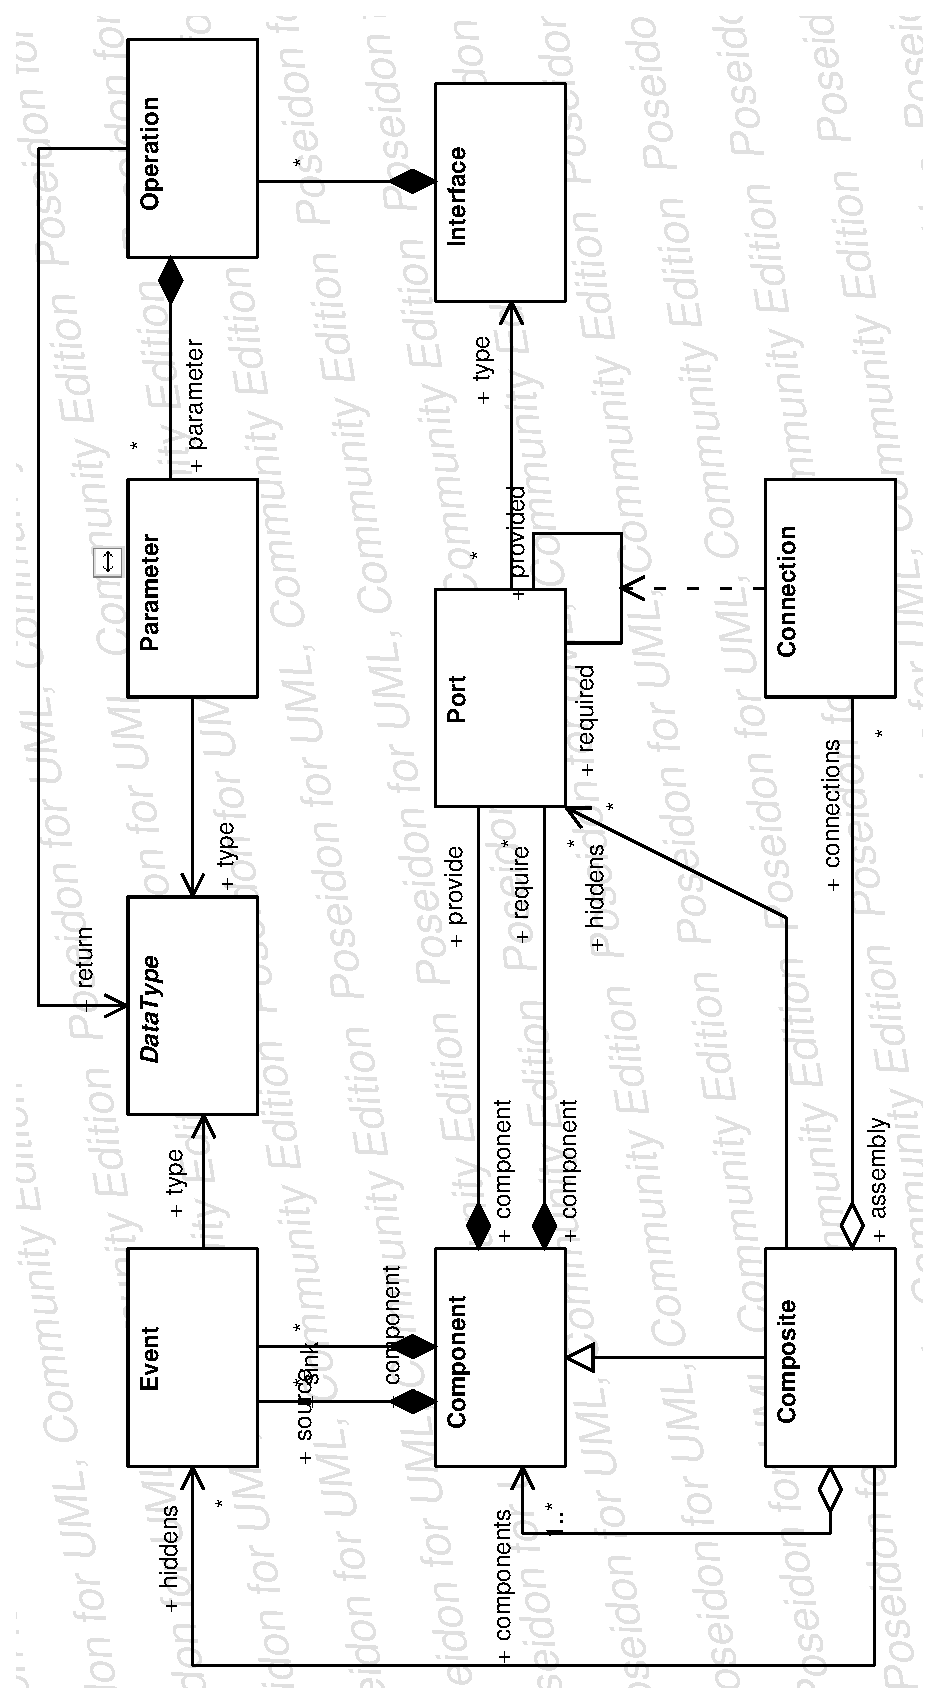
\includegraphics[angle=-90,width=\textwidth]{figures/fig-mmcomposant.eps}
    \caption{M\'eta-mod\`ele de composants \textsf{FIDL}}
    \label{fig-mmcomposants}
\end{figure}


\subsection{Interfaces \& ports synchrones}

Une interface \textsf{FIDL} d\'efinit un \emph{protocole} de communication entre deux
composants au travers d'une \emph{connexion}, protocole d\'efini sous la forme d'\emph{op\'erations}  --- ou
m\'ethodes --- et d'\emph{attributs} susceptibles de g\'en\'erer des
appels, des retours et des exceptions. Une op\'eration est identifi\'ee
par son nom, le type et la modalit\'e ---  \texttt{in},
\texttt{inout} et \texttt{out} --- de ses param\`etres. 
Le cas des attributs est un cas particulier : ils ne sont accessibles que
par l'interm\'ediaire d'\emph{accesseurs} et de \emph{mutateurs}, c'est
\`a dire des op\'erations implicites nomm\'ees \texttt{getXXX} et
\texttt{setXXX} respectivement pour chaque attribut \texttt{XXX}. 

Une interface peut h\'eriter d'une ou plusieurs autres interfaces ce qui
ne pose pas de probl\`emes de r\'esolution statique : l'absence de corps
de m\'ethode n'introduit pas les conflits d'h\'eritages typiques des
langages \`a h\'eritage multiple tels que le \textsf{C++}. L'h\'eritage pose
toutefois un certain nombre de probl\`emes lorsque l'on prend en compte
la sp\'ecification formelle des interfaces et cette question sera
\'etudi\'ee dans la section \ref{sec:heritage-comportemental} du chapitre \ref{cha:composition}.

Une interface d\'efinit le \emph{type} d'une facette ou d'un
r\'eceptacle susceptibles d'\^etre d\'eclar\'es dans la
d\'efinition d'un composant. Ce type est un \'el\'ement permettant de
v\'erifier la validit\'e d'une connexion entre facette et r\'eceptacle : la
facette doit \^etre un sous-type du type du r\'eceptacle pour que la
connexion soit, au moins syntaxiquement, consid\'er\'ee comme l\'egale. 

Enfin, il est possible de d\'efinir des modalit\'es de connexion pour
chaque facette :
\begin{itemize}
\item \emph{unique} si le port ne peut \^etre utilis\'e que par un et un
  seul composant \`a la fois  (c'est le cas par d\'efaut) ;
  \item \emph{single} si le m\^eme port peut \^etre partag\'e par
  plusieurs composants connect\'es ;
\item \emph{multiple} si chaque composant connect\'e \`a ce port est
  \emph{isol\'e} des autres composants. Le port est en fait multiplex\'e
  et chaque connexion poss\`ede son propre \'etat conversationnel
  ind\'ependant de toutes les autres connexions.
\end{itemize}

Cette notion de \emph{modalit\'e} d'interface permet d'int\'egrer dans la
sp\'ecification les typologies de mod\`ele d'ex\'ecution du
composant qui sont pr\'ecis\'ees dans le cas du \textsf{CCM} et
de \textsf{J2EE} par des descriptions externes. On dispose ainsi
des notions famili\`eres d'objet \emph{session}, \emph{processus} ou
\emph{m\'ethode}, transpos\'ees des composants \`a  leurs ports et
disponibles dans le mod\`ele, et un m\^eme composant pourra donc offrir
simultan\'ement des facettes de diff\'erentes modalit\'es. Par la
suite, nous consid\'ererons uniquement le cas des facettes
\emph{unique}. Le cas des facettes \emph{single} introduit le partage de facettes entre
plusieurs composants et ruine la possibilit\'e de composer les
composants en ne tenant compte que de leur \emph{topologie de connexion}, il 
impose donc pour valider une architecture de v\'erifier le respect des
contrats en fonction de l'ensemble des composants connect\'es et ne
permet pas de raisonner uniquement de mani\`ere
compositionnelle. C'est une version du probl\`eme bien connu  
de l'\emph{aliasing}. En ce qui concerne les facettes \emph{multiple},
leur traitement n'introduit pas de difficult\'e conceptuelle
suppl\'ementaire mais est techniquement assez complexe : compte tenu
du fait que le syst\`eme que nous d\'ecrivons et la s\'emantique
des langages de traces est d\'ej\`a relativement touffue, nous avons
choisi de reporter le traitement de ce cas \`a des travaux ult\'erieurs.

\subsection{\'Ev\'enements \& ports asynchrones}

Les ports d'\'ev\'enements asynchrones, \emph{sources} et \emph{puits} sont
typ\'es par le type d'\'ev\'enement --- un objet-valeur --- qu'ils sont
susceptibles de consommer ou de produire. Ces objets-valeur --- ou
\texttt{eventtype} --- sont des structures de donn\'ees arbitrairement
complexes. En \textsf{IDL3}, un \texttt{eventtype} 
peut d\'efinir des attributs, des op\'erations, des types export\'es,
etc... comme n'importe quel autre espace de nommage. C'est en fait un
v\'eritable \emph{objet}, au sens des langages objets, dont l'\'etat
peut-\^etre observ\'e et \'eventuellement modifi\'e par n'importe quel
\'el\'ement du syst\`eme. 

Dans un premier temps, nous ne nous int\'eresserons aux \'ev\'enements que
sous l'angle d'une structure de donn\'ees particuli\`ere transport\'ee par des
ports asynchrones. 

\subsection{Connexion \& composition}

Un composant ne peut \^etre fonctionnel que si tous ses r\'eceptacles sont
correctement connect\'es \`a une facette, et si toutes ses sources 
d'\'ev\'enements sont connect\'ees \`a un puits
d'\'ev\'enements. Les services synchrones et asynchrones requis par
le composant sont en effet suppos\'es \^etre utilis\'es par
celui-ci \`a un moment ou un autre pour qu'il soit en mesure de
rendre les services qu'il fournit. Une connexion
est une relation un-vers-un  entre ports de composants. 

Un \emph{composite} est un ensemble de composants  partiellement ou
totalement inter-connect\'es, autrement dit un composant r\'ealis\'e par
\emph{assemblage} de plusieurs autres composants. Nous utiliserons le
terme de Un \emph{syst\`eme} pour d\'esigner un ensemble quelconque
de ports sans identit\'e pr\'ecise. 

Du point de vue de la sp\'ecification, un composite peut permettre de
masquer certaines facettes et a pour effet principal de rendre
inobservable l'ensemble des messages transitant par les connexions
r\'ealis\'es entre ses composants.  
On notera que la notion de composite, conceptuellement simple et
  \'el\'egante, n'est pas aujourd'hui prise en compte 
  directement dans les plate-formes existantes, \`a l'exception de
  \textsf{.Net} sous la forme des \emph{assembly}. Elle est par contre essentielle dans
la plupart des mod\`eles formels \'etudi\'es. 

Les connexions sont r\'ealis\'ees durant la phase de d\'eploiement et peuvent normalement
\'evoluer au court du cycle de vie du composant. Nous
consid\'erons ici le cas simple o\`u les connexions des composants sont
  \'etablies au \emph{d\'eploiement} et ne sont plus modifi\'ees jusqu'\`a l'arr\^et du
  syst\`eme. 

\subsection{Ex\'ecution \& Communication}

Ainsi que nous l'avons dit pr\'ec\'edemment, aucune hypoth\`ese n'est faite
quant aux flots d'ex\'ecution des composants. Nous nous int\'eressons
uniquement aux messages \'echang\'es entre les diff\'erents composants au
travers de leurs connexions. Ces messages sont nomm\'es et contiennent
des donn\'ees primitives ou structur\'ees selon le typage des interfaces
du port concern\'e. De plus, ces messages identifient de mani\`ere
unique l'\'emetteur et  le r\'ecepteur.

Le m\'edium de communication est suppos\'e fiable : tous les messages
envoy\'es atteignent leur destination en un temps fini, mais nous ne
supposons rien quant \`a l'ordre d'arriv\'ee des messages entre
diff\'erentes connexions qui peuvent \^etre arbitrairement entrelac\'es. Sur une m\^eme connexion
point-\`a-point, l'ordre des messages est toutefois suppos\'e maintenu entre
l'\'emetteur et le r\'ecepteur. 

Les \'ev\'enements observables d'un syst\`eme sont les messages \'echang\'es
entre les composants de ce syst\`eme au travers de leurs connexions,
sachant que l'\'emission et la r\'eception d'un message constituent deux
\'ev\'enements distincts observ\'es \`a chacun des points de la
connexion. Chaque composant poss\`ede son propre point de vue sur le
syst\`eme et donc ne peut observer qu'un sous-ensemble des \'ev\'enements
globaux, en l'occurrence les messages re\c{c}us et \'emis sur les connexions
auxquelles il participe.

\section{Le langage \textsf{FIDL}}
\label{sec:syntaxe-fidl}
Le langage \textsf{FIDL} est  construit par agr\'egation de plusieurs langages,
chacun destin\'e \`a d\'efinir une partie du syst\`eme sp\'ecifi\'e :
\begin{enumerate}
  \item le langage \textsf{IDL3}, d\'efini dans le \textsf{CORBA Component
      Model}\cite{ccmspec}, permet de d\'ecrire les
    \emph{interfaces} et la structure des \emph{types} de donn\'ees
      permettant \`a un syst\`eme de communiquer avec son environnement. Cette description ind\'ependante
    de tout langage de programmation est destin\'ee \`a \^etre
    \emph{projet\'ee} dans un langage sp\'ecifique puis compl\'et\'ee par
    l'environnement d'ex\'ecution ;
  \item le langage \textsf{FIDL} proprement dit, qui d\'ecrit le
    comportement des interfaces et composants \textsf{IDL3}  en termes d'ensemble de traces ;
  \item le langage \textsf{Jaskell}, un langage fonctionnel sans effets de bord \`a \'evaluation
    paresseuse, sous-ensemble de \textsf{Haskell
      98}\cite{h98report}, permettant de d\'efinir des
    fonctions sur les types \textsf{IDL3} et donc de pr\'eciser le contenu
    des messages circulant dans le syst\`eme. 
\end{enumerate}
La partie sp\'ecification --- \textsf{FIDL} et \textsf{Jaskell} --- est
incluse dans la description \textsf{IDL3} sous la forme de
commentaires et est donc transparent pour les
outils existants de manipulation de mod\`eles \textsf{IDL3}. L'ensemble de la sp\'ecification couvre donc  les \'el\'ements \emph{structuraux},
\emph{comportementaux} et \emph{calculatoires} du syst\`eme d\'ecrit.

L'objectif du langage \textsf{FIDL} est que, en utilisant une seule et m\^eme
notation, l'on puisse tester, valider et v\'erifier des composants et assemblages
selon diff\'erentes technologies, voire m\^eme entre plate-formes
h\'et\'erog\`enes. La notation \textsf{IDL3} est celle qui nous a paru
offrir la meilleure couverture des concepts que nous souhaitions voir
appara\^{\i}tre et nous l'avons donc choisie comme outil de  description
structurelle d'une sp\'ecification. On verra au chapitre
\ref{cha:methodes--outils} comment ce langage est implant\'e concr\`etement
dans un outil et comment des applications vers diverses plateformes
techniques peuvent \^etre mises en \oe uvre.

% \begin{figure}[h]
% \includegraphics{../figures/archi-general.eps}
% \caption{Architecture \textsf{FIDL}.}
% \label{fig-archi-general}
% \end{figure}


La notation \textsf{FIDL} s'appuyant sur le langage \textsf{IDL3},
nous en rappelerons ici les principaux \'el\'ements avant de
d\'etailler la  
partie proprement originale de \textsf{FIDL}. Le lecteur souhaitant plus de
d\'etails pourra consulter les documents de r\'ef\'erence de l'\textsf{OMG}
tels que \cite{ccmspec,corbaspec}. La grammaire EBNF compl\`ete du
langage \textsf{FIDL} est donn\'ee en annexe
\ref{cha:grammaire-fidl}.

L'ensemble de ces langages est fondu dans la s\'emantique sous la
forme d'un seul et m\^eme syst\`eme formel  d\'etaill\'e dans la
section \ref{section-semantique}. L'utilisation de ces syntaxes
particuli\`eres est donc tout \`a fait contingente et nous avons la
possibilit\'e de substituer toute notation \'equivalente pour l'un
ou l'autre de ces \'el\'ements. Par exemple, on peut imaginer
d'embarquer les sections comportementales et calculatoires de \textsf{FIDL}
dans un mod\`ele \textsf{UML} respectant le m\'eta-mod\`ele
repr\'esent\'e dans la figure \ref{fig-mmcomposants} ou de remplacer
le langage fonctionnel \textsf{Jaskell} par un --- fragment d'un --- autre langage
d'expressions tel que \textsf{JML}\cite{jmlnotation} ou
\textsf{OCL}\cite{ocl20spec}. 

\subsection{\textsf{IDL3}}

Le langage de description d'interface \textsf{IDL} de \textsf{CORBA} et son extension propre au
mod\`ele de composant \textsf{CCM} est une \emph{lingua franca} entre langages
de programmation et syst\`emes de communication permettant d'assurer une
interop\'erabilit\'e au niveau de granularit\'e le plus fin, celui des
donn\'ees et des appels de proc\'edures distants, tout en assurant un
minimum de structuration orient\'ee-objet. Un fichier IDL a vocation
d'\^etre utilis\'e par un outil qui en projettera le contenu dans un
langage sp\'ecifique pour assurer la communication avec un \emph{Object
  Request Broker} donn\'e.

Le langage \textsf{IDL3} permet de d\'efinir les \'el\'ements suivants :
\begin{enumerate}
  \item des \emph{modules}, espaces de nommages ind\'ependants et arborescents
  ;
\item  des \emph{types} de donn\'ees vari\'es : types num\'eriques,
  structures, unions ou \'enum\'erations ;
\item des \emph{interfaces}, pouvant h\'eriter d'une ou plusieurs autres
  interfaces, chaque   interface d\'efinissant :
  \begin{enumerate}
    \item des \emph{op\'erations} ou m\'ethodes, avec leurs
    param\`etres, la modalit\'e des param\`etres --- \texttt{in}, \texttt{out}, \texttt{inout},
    leur type de retour, des exceptions \'eventuelles,
  \item des \emph{attributs} manipulables au travers d'accesseurs et
  de mutateurs,
\item des \emph{types} ;
  \end{enumerate}
\item des \emph{composants} d\'efinissant  des \emph{ports},
  facettes, r\'eceptacles, sources, puits ;
\item des maisons des composants --- fabriques ---  permettant de
  d\'efinir en sus des op\'erations et attributs usuels des op\'erations de
  recherche --- \emph{finder} --- et de construction ---
  \emph{factory} --- de composants ;
\item des types d'\emph{exceptions} contenant \'eventuellement des
  donn\'ees complexes ;
\item des objets-valeurs --- \texttt{valuetype} ---, c'est \`a dire des classes
  avec leurs op\'erations, attributs, types, ... dont les instances sont
  pass\'ees par valeur et non par r\'ef\'erence.
\end{enumerate}

Pour des raisons de coh\'erence du mod\`ele,
nous avons choisi de ne pas tenir compte de certains aspects du
langage \textsf{IDL3}, en particulier :
\begin{itemize}
  \item la possibilit\'e pour les composants d'implanter des
  interfaces. Il nous semble que
  cette possibilit\'e rel\`eve de \og l'h\'eritage alimentaire\fg~
  et n'est pr\'esente que pour des raisons de compatibilit\'e ;
\item la complexit\'e des objets-valeur qui sont, pour ce qui nous
  concerne, trait\'es comme de simples structures.
\end{itemize}

Une sp\'ecification \textsf{IDL3} est normalement accompagn\'ee de
l'implantation correspondante et de fichiers de description
d'assemblage et de d\'eploiement. Nous  discuterons de ce probl\`eme
dans le chapitre \ref{cha:methodes--outils} consacr\'e \`a l'outil
\textsf{FIDL}  o\`u nous verrons que ces informations propres aux 
composants\textsf{ CCM } seront utitlis\'ees dans le cadre du test.

\subsection{D\'eclaration}

Une sp\'ecification \textsf{FIDL} est incluse en tant que commentaire dans une
description d'interface, de composant ou de maison de composant
\textsf{IDL3}. Cette sp\'ecification est subdivis\'ee en trois
parties :
\begin{enumerate}
  \item une premi\`ere partie --- optionelle --- d\'eclarative introduisant les noms et
    types des fonctions utilis\'ees dans l'expression \textsf{FIDL}
    proprement dite ;
  \item une seconde partie qui est l'expression \textsf{FIDL} ;
  \item une troisi\`eme partie optionelle comprenant les d\'efinitions
    de fonctions pr\'ec\'edemment d\'eclar\'ees. 
\end{enumerate}

Les sections 1 et 3  concernant les fonctions permettent de
d\'eclarer et d\'efinir
des fonctions auxiliaires sans effets de bord pour calculer les
valeurs des donn\'ees transmises dans les messages. Le fait que la
d\'eclaration soit s\'epar\'ee de la d\'efinition permettra \`a
terme de changer le langage d'implantation des fonctions auxiliaires.

\subsection{Interfaces}
\label{sect-interfaces}

La sp\'ecification d'une interface d\'efinit un \emph{contrat}, au sens de \cite{meyer}, entre toute
\emph{facette} typ\'ee par cette interface et tout composant utilisant une
facette de ce type. Ce contrat est divis\'e en trois parties : une
partie syntaxique d\'efinissant les structures de messages \'ecrite
en \textsf{IDL3} ; une
partie protocolaire d\'ecrivant les s\'equences d'\'echanges de messages
autoris\'ees par cette interface, c'est \`a dire l'ensemble de
traces repr\'esentant le protocole d'utilisation et d'implantation de
l'interface ; une partie calculatoire d\'efinissant
des fonctions utilis\'ees pour l'\'evaluation des valeurs
\'echang\'ees \'ecrite actuellement dans le langage \textsf{Jaskell}. On
notera que le contrat s'applique \`a l'\emph{interface} et non \`a
un port donn\'e et donc que sa mise en \oe uvre concr\`ete d\'epend
des modalit\'es de connexion du port typ\'e par l'interface : une
facette \texttt{single} qui est partag\'ee entre plusieurs connexions
voit les messages de toutes ses connexions arbitrairement
entrelac\'es, ce qui n'est pas le cas pour une facette
\texttt{multiple} laquelle est instanci\'ee de mani\`ere
ind\'ependante \`a chaque connexion.

L'exemple \ref{fig-ex1} d\'ecrit une interface simple offrant trois
m\'ethodes sans param\`etres ni valeur de retour et sp\'ecifiant un
comportement de type \og session \fg : l'utilisateur doit commencer par
appeler la m\'ethode \texttt{ouvrir}, puis il peut faire un nombre
quelconques d'appels \`a \texttt{m} et il doit terminer avec un appel \`a
\texttt{fermer} avant de pouvoir recommencer. 

\begin{figure}[h]
\centering
\begin{lstlisting}
module Acces {   
  interface Controle {
    void ouvrir ();
    void m ();
    void fermer ();
    /*** FIDL
      (ouvrir()m()*fermer())*
    */
  }
...
}
\end{lstlisting}
    \caption{Interface (sans donn\'ees).}
    \label{fig-ex1}
\end{figure}

Une expression
\textsf{FIDL} prend la forme d'une \emph{expression rationnelle} dont les lettres sont
des expressions d\'enotant des messages. On retrouve les op\'erateurs
usuels que sont la concat\'enation, l'alternative (\texttt{+}), le
produit de m\'elange ($\parallel$) et l'it\'eration ($\star$) et comme on peut s'y
attendre, les parenth\`eses permettent de grouper les expressions et de
modifier l'ordre de pr\'ec\'edence usuel des op\'erateurs.

Un message  $\rightarrow m(x_0,\dots,x_n)$ d\'enote un appel
de m\'ethode $m$ avec des param\`etres \texttt{in}- et \texttt{inout}- $x_0,\dots,x_n$ ;
un message $\leftarrow m(x_0,\dots,x_n:x)$ d\'enote un retour d'appel de
m\'ethode $m$ avec les param\`etres \texttt{inout}- et \texttt{out}- $x_0,\dots,x_n$ et
une valeur de retour $x$.  Les valeurs des param\`etres et de
retour des messages peuvent \^etre soit des valeurs litt\'erales, soit des
variables d\'eclar\'ees dans une expression de liaison englobante, soit un
caract\`ere \emph{joker} \verb+'_'+. La
notation abr\'eg\'ee $m(x_1,\dots,x_n:x)$ comprenant l'appel et le retour
pour une m\'ethode $m$ est autoris\'ee dans la mesure o\`u il n'y a
pas d'ambigu\"{\i}t\'e  possible sur les param\`etres --- c'est \`a
dire qu'il n'y a pas de param\`etres en mode \texttt{inout} ou que
leurs valeurs est sans importance dans l'expression (\verb+_+).

Une exception lev\'ee par une m\'ethode est d\'enot\'ee  $\leftarrow
m<E[x_0,\dots,x_n]>$ o\`u $E$ est le type de l'exception et
$x_0,\dots,x_n$ les valeurs des champs du type $E$.

L'exemple \ref{fig-exifaceaccount} est un peu plus complexe puisqu'il introduit
la notion de fonction et de \emph{contraintes} sur les valeurs des messages.
Une expression de contrainte $x_1:P_1(x_1);\dots;x_n:P_m(x_m)\ \mathtt{in}\ E$
a pour effet :
\begin{enumerate}
  \item d'introduire dans la port\'ee de l'expression $E$ les variables
  d\'eclar\'ees $x_1,\dots,x_n$  ;
\item de d\'efinir des contraintes $P_i(x_i)$ sur les valeurs possibles de ces
  variables sous la forme d'un pr\'edicat logique liant une variable
  $x_i$. Ce pr\'edicat peut \'eventuellement \^etre omis auquel cas
  il est consid\'er\'e comme la constante \textbf{true}.
\end{enumerate}
Le type de chaque variable peut normalement \^etre inf\'er\'e de
son contexte par le \emph{v\'erificateur de types}, car chaque
variable utilis\'ee correspond \`a un param\`etre typ\'e d'une m\'ethode. Si ce n'est pas
le cas, l'ambigu\"{\i}t\'e pourra \^etre lev\'ee en ins\'erant une
notation de type $x\twocol T$ apr\`es la d\'eclaration de la variable. 

Les variables introduites sont li\'ees dans l'environnement apr\`es
leur d\'efinition ce qui les rend disponibles pour les expressions de
contraintes suivantes mais interdit les expressions r\'ecursives,
c'est \`a dire les expressions contraignant deux  variables et se
faisant mutuellement r\'ef\'erence. De
fait, la notation  $x_1:P_1(x_1);\dots;x_n:P_m(x_m)\ \mathtt{in}\ E$
est une facilit\'e syntaxique pour $(x_1:P_1(x_1)\ \mathtt{in}\
(x_2:P_2(x_2) \ \mathtt{in}\ \dots (x_n:P_m(x_m)\ \mathtt{in}\ E))$.
Les contraintes sont des expressions fonctionnelles quelconques de
type bool\'een. 
Ce pr\'edicat est \'evalu\'e \`a chaque utilisation de la
variable avec la valeur effective qu'elle poss\`ede au moment de
l'\'evaluation, valeur qui d\'epend du contenu des
messages. 

\begin{figure}[htbp]
    \centering
\begin{lstlisting}
  interface Accounts {
    long    balance (in long accountNo) ;
    boolean withdraw (in long accountNo, in long amount) ;
    void    deposit (in long accountNo,in long amount) ;
    
      /*** 
        header
          -- retourne le solde courant pour un numero de compte donne
          bal : Trace,long -> long;
        FIDL
         (
         ((n in ->balance(n) (s : s == bal(Trace,n) in <-balance(s)))) +
         (n,m in ->withdraw(n,m) (ko : ko == (m <= bal(Trace,n)) in <-withdraw(ko))) +
         deposit(_,_) 
         )*

        body
        bal (~->withdraw(num,somme) : ~<-withdraw(True) : h) numc = 
            if (num == numc) then (bal h num) - somme else (bal h num); 
        bal (~->transfer(num,somme,to) : ~<-transfer(True) : h) numc = 
            if (num == numc) then (bal h num) - somme else (bal h num); 
        bal (~->depot(num,somme)  : h) numc = 
            if (num == numc) then (bal h num) + somme else (bal h num);
        bal (_ : h) num = bal h num;
        bal [] num = 0
                
       */
   };   
\end{lstlisting}
        \caption{Exemple de sp\'ecification \textsf{FIDL} : interface Accounts}
    \label{fig-exifaceaccount}
\end{figure}

L'exemple de la figure \ref{fig-exifaceaccount} sp\'ecifie le
comportement d'une interface permettant de r\'ealiser des
op\'erations sur des comptes bancaires. La
sp\'ecification de l'interface \texttt{Account} est divis\'ee en
trois parties dont la signification informelle est la suivante : 
\begin{itemize}
  \item la section principale est introduite par le mot-cl\'e
    \texttt{FIDL}, c'est elle qui contient la sp\'ecification
    comportementale de l'interface, c'est \`a dire une expression du
    langage \textsf{FIDL}. Dans le cas pr\'esent, cette expression se r\'eduit \`a
    \texttt{balance()* + withdraw()* + deposit()*}  si l'on ne tient pas
    compte du contenu des messages, ce qui signifie que les trois
    m\'ethodes sont totalement ind\'ependantes --- peuvent \^etre appel\'ees
    dans n'importe quel ordre. L'introduction de variables et
    d'expressions de contraintes permet de pr\'eciser le r\'esultat de
    l'appel de m\'ethode sur cette interface, en l'occurence le fait
    qu'un d\'ebit n'est autoris\'e que si son montant est inf\'erieur au solde
    courant (calcul\'e par la fonction \texttt{bal}), qu'un d\'ep\^ot est
    toujours autoris\'e quelqu'en soit le montant et que la m\'ethode
    \texttt{balance} calcule le solde courant du compte ;
  \item la section \texttt{body} contient la d\'efinition de la ou des fonctions
    utilis\'ees dans la partie principale de la sp\'ecification. Ces
    fonctions peuvent \^etre th\'eoriquement \'ecrites dans n'importe quel
    langage sans effet de bord. Dans la pratique, on utilisera un
    sous-ensemble du langage \textsf{Haskell}. La fonction \texttt{bal} calcule
    le solde courant pour un num\'ero de compte donn\'e en fonction
    de l'historique des retraits et des d\'ep\^ots intervenus sur ce
    compte. Dans l'expression du langage de traces de l'interface, la
    fonction est utilis\'ee pour contraindre les valeurs possibles
    de certaines variables, en l'occurence la valeur de retour des
    m\'ethodes \texttt{withdraw} et \texttt{deposit}, en fonction du
    num\'ero de compte pour lequel la m\'ethode est invoqu\'ee et
    de la trace courante de l'interface d\'enot\'ee par la variable
    globale \texttt{Trace} ;
  \item la section \texttt{header} permet de s'abstraire du langage
    concret utilis\'e pour \'ecrire des fonctions. On y d\'eclare uniquement le type des
    fonctions selon une syntaxe normalis\'ee, les types utilis\'es
    \'etant ceux du langage \textsf{IDL3}.
\end{itemize}

Lorsque la sp\'ecification d'une interface n'est pas explicitement
donn\'ee, elle est inf\'er\'ee automatiquement \`a partir de sa
signature : pour toute interface $I$ offrant les m\'ethodes
$m_1,m_2,\dots,m_n$, le langage induit de l'interface est l'ensemble
des appels-retours possibles des m\'ethodes de $I$ sans contrainte
sur les param\`etres ni ordonnancement des m\'ethodes.

\subsection{Composants}

Comme dans le cas des interfaces, les sp\'ecifications \textsf{FIDL} des
composants sont ins\'er\'ees sous forme de commentaires \`a la fin de la
description \textsf{IDL3}. Cette sp\'ecification est un peu plus compliqu\'ee car
elle d\'ecrit les interactions entre les diff\'erents services requis et
offerts par le composant, la structure g\'en\'erale est cependant la
m\^eme. Le composant est sens\'e respecter les sp\'ecifications des
interfaces des facettes qu'il offre, ces sp\'ecifications font donc
implicitement partie de la sp\'ecification du composant. 

L'expression d'un composant est une conjonction de plusieurs expressions que l'on peut
voir comme des descriptions de parties du comportement du
composant. Cette op\'eration de \og composition\fg{} est not\'ee
\texttt{and} et n'apporte pas de r\'eel pouvoir d'expression
suppl\'ementaire  (\emph{cf.} section \ref{section-semantique}) mais plut\^ot des facilit\'es d'\'ecriture appr\'eciables : les
comportements peuvent \^etre d\'ecrits comme une conjonction de vues
diff\'erentes.

Un \'ev\'enement d'un composant contient plus d'informations que celui
d'une interface : le composant re\c{c}oit l'\'ev\'enement par un port et donc
le nom du port devient partie int\'egrante de l'\'ev\'enement car
un composant peut offrir ou requ\'erir plusieurs ports d'un m\^eme type. D'autre part,
les composants peuvent \'echanger des messages synchrones comme des
messages asynchrones et les messages asynchrones peuvent \^etre
entrelac\'es. On
utilise \`a nouveau les symboles $\rightarrow$ et $\leftarrow$ pour
d\'esigner les appels et retour de m\'ethodes et le point lorsqu'il s'agit
d'un appel suivi du retour correspondant : $a\rightarrow m(),
a\leftarrow m(), a.m()$. 

%% Notons que, dans le cas des ports \texttt{multiple}, le \emph{nom} du port
%% repr\'esente \emph{une} instance de ce port, utilis\'ee au travers
%% d'une connexion, alors que dans le cas de facettes \texttt{single}, ce nom d\'esigne
%% toujours \emph{une} instance du port mais utilis\'ee au travers de
%% \emph{plusieurs} connnexions. Les cons\'equences sur l'ensemble de
%% traces r\'esultant de l'expression sont importantes. 

La figure \ref{fig-excompbkaccount} est un exemple de composant
\texttt{BankAccount} offrant une interface \texttt{Accounts},
\'emettant des messages de type \texttt{Offer} et utilisant une
interface \texttt{Banker} suppos\'ee offrir une m\'ethode
\texttt{alert()}. Cette sp\'ecification pr\'ecise que :
\begin{itemize}
  \item chaque fois qu'un d\'ep\^ot sup\'erieur \`a 100 est effectu\'e, un
  message d'alerte est transmis au banquier ;
\item lorsqu'un d\'ebit est refus\'e, c'est \`a dire lorsque la
  m\'ethode \texttt{withdraw} retourne la valeur
  \texttt{false}, une offre de cr\'edit est adress\'ee au client (\'emission
  d'un message asynchrone de type \texttt{Offre}). 
\end{itemize}

Par ailleurs, le composant doit respecter la sp\'ecification de
l'interface \texttt{Accounts} dont la sp\'ecification est implicitement
ajout\'ee \`a la sienne. 

\begin{figure}[htbp]
    \centering
\begin{lstlisting}
composant BankAccount {
  provides Accounts a;
  uses Banker b;
  emits Offer o;
  /*** FIDL
    ((n,m:m<=100 in a->deposit(n,m)a<-deposit()) +
     (n,m:m > 100 in a->deposit(n,m) b.alert() a<-deposit()))*
    and 
     (a.withdraw(_,_:true) + 
      a->withdraw(_,_) o[] a<-withdraw(:false))*
  */
}
\end{lstlisting}
        \caption{Exemple de sp\'ecification \textsf{FIDL} : composant \textsf{BankAccount}}
    \label{fig-excompbkaccount}
\end{figure}

\subsection{Grammaire}
\label{sec:grammaire}
La grammaire compl\`ete du langage est donn\'ee dans l'annexe
\ref{cha:grammaire-fidl}, nous en donnons dans la figure
\ref{fig-syn-fidl} une version
abr\'eg\'ee d\'efinissant uniquement la syntaxe des expressions de
comportement pour faciliter la lecture des exemples et d\'efinitions
de ce chapitre. La partie gauche d\'ecrit la syntaxe des
expressions \textsf{FIDL} dites \'el\'ementaires pour une sp\'ecification d'interface. La partie droite d\'ecrit la syntaxe abstraite des
expressions de contraintes sur des variables.

\begin{figure}[htbp]
\begin{minipage}[t]{.45\textwidth}
    \begin{equation}
\label{eq:syn-fidl}\begin{array}{ccl}
        Expr &\quad\rightarrow\quad& Expr Expr \mid Expr^* \mid \\
        && Expr + Expr \mid (Expr) \mid \\
        && Expr \parallel Expr \mid \\
&&(Ctr\ \mathbf{in}\ Expr) \mid \\
        && Msg \mid \mathtt{void}\\
        Msg &\quad\rightarrow\quad& \leftarrow m(Out) \mid \\
        && \rightarrow m(In) \mid m(Out) \\
        In &\quad\rightarrow\quad& \epsilon \mid Param \\
        Param &\quad\rightarrow\quad& Atom \mid Atom,Param \\
        Atom &\quad\rightarrow\quad& x \mid l \\
        Out &\quad\rightarrow\quad& \epsilon \mid In\ Ret \\
        Ret &\quad\rightarrow\quad& \epsilon \mid : Atom \\
\end{array}
\end{equation}
\end{minipage}
\begin{minipage}[t]{.45\textwidth}
    \begin{equation}
\label{eq:syn-constraint}\begin{array}{ccl}
Ctr &\quad\rightarrow\quad& x : Pred \\
Pred &\quad\rightarrow\quad& \mathtt{true} \mid \mathtt{false} \mid \\
&&Pred \vee Pred \mid \neg{}Pred \mid p
(x,Fun)  \\
Fun &\quad\rightarrow\quad& f(Par) \mid l \\
Par &\quad\rightarrow\quad& Par,y  \mid y \mid Fun \\
\end{array}
\end{equation}
\end{minipage}\centering

\caption{Syntaxe des expressions \textsf{FIDL} (interfaces)}
\label{fig-syn-fidl}
\end{figure}

Les symboles $x$,$y$ d\'esignent des terminaux repr\'esentant une
variable, $p$ est un symbole terminal repr\'esentant un pr\'edicat,
$l$ est un symbole terminal repr\'esentant un litt\'eral et  $f$ un symbole
de fonction n-aire. Pour faciliter l'\'ecriture des contraintes, on
permettra d'\'ecrire 
$$
(x:P(x),y:P(y)\ \mathbf{in}\ E)
$$
au lieu  de
$$
(x:P(x)\ \mathbf{in}\ (y:P(y)\ \mathbf{in}\ E)).
$$

Par ailleurs, on autorise l'utilisation du symbole \_ comme \og
joker\fg. Pour chaque utilisation de ce symbole, on substitue
implicitement dans l'expression une variable $x$ au symbole \_ et on
lie $x$ par une contrainte qui est toujours vraie : 
$$
\leftarrow m(\_) \Leftrightarrow (x:\mathbf{true}\ \mathbf{in}\ m(x)).
$$

Un composant est sp\'ecifi\'e par un
nombre quelconque d'expressions \'elementaires reli\'ees par
l'op\'erateur \textbf{and}. De plus l'identit\'e des ports mis en
\oe uvre doit \^etre pr\'ecis\'ee et un composant peut \'emettre
et recevoir des messages au travers de ports asynchrones. La grammaire
des expressions \textsf{FIDL} pour les composants est pr\'esent\'ee dans la
figure \ref{fig-syn-fidl-comp}.

\begin{figure}
    \begin{equation}
        \label{eq:syn-fidl-comp}\begin{array}{ccl}
            Comp &\quad\rightarrow\quad& Comp \mathbf{~and~} Expr \mid Expr \\
            Expr &\quad\rightarrow\quad& Expr Expr \mid Expr^* \mid Expr + Expr \mid Expr \parallel Expr \mid \\
            && (Expr) \mid (Ctr\mbox{~in~} Expr) \mid Msg\\
            Msg &\quad\rightarrow\quad& n \leftarrow m(Out) \mid n
            \rightarrow m(In) \mid n \leftarrow m(Out) \mid \\ 
            &&n \leftarrow Event \mid n \rightarrow Event \\
            Event &\quad\rightarrow\quad& t [ In ] \\
            In &\quad\rightarrow\quad& \epsilon \mid Param \\
            Param &\quad\rightarrow\quad& Atom \mid Atom,Param \\
            Atom &\quad\rightarrow\quad& x \mid l  \\
            Out &\quad\rightarrow\quad& \epsilon \mid In Ret \\
            Ret &\quad\rightarrow\quad& \epsilon \mid : Atom \\
        \end{array}
    \end{equation}
    \caption{Syntaxe des expressions \textsf{FIDL} (composants)}
    \label{fig-syn-fidl-comp}
\end{figure}

Dans l'exemple de la figure \ref{fig-excompbkaccount}, les messages
concernant la m\'ethode \texttt{balance} seront conserv\'es dans le
langage du composant car ils ne font pas partie de l'alphabet de
synchronisation. Par contre, cette d\'efinition oblige \`a
sp\'ecifier totalement le comportement du composant pour les messages
faisant partie de l'alphabet de ses expressions, comme on le voit pour
les m\'ethodes \texttt{withdraw} et \texttt{deposit}.
    
\section{Exemples} 
\label{sec:exemples}
\subsection{Un guichet  automatique de banque}

Nous d\'etaillons dans cette section un exemple complet de
sp\'ecification de composants \textsf{FIDL}, un syst\`eme de gestion de
\emph{Guichet Automatique de Banque}. La structure g\'en\'erale du mod\`ele
est d\'ecrite dans la figure \ref{fig-exbanque} : le module
\texttt{Banque} d\'ecrit un certain nombres d'interfaces et deux
composants : un composant \texttt{ATM} --- \emph{Automatic Teller Machine}
--- qui est une repr\'esentation de la machine physique utilis\'ee
par un client et un composant \emph{Bank}, fournissant des ports de
type \texttt{Account}. L'architecture du syst\`eme est
sch\'ematis\'ee dans la figure \ref{fig-gab}, seule la partie
concernant le guichet automatique \'etant d\'ecrite plus pr\'ecis\'ement.

\begin{figure}[htbp]
    \centering
    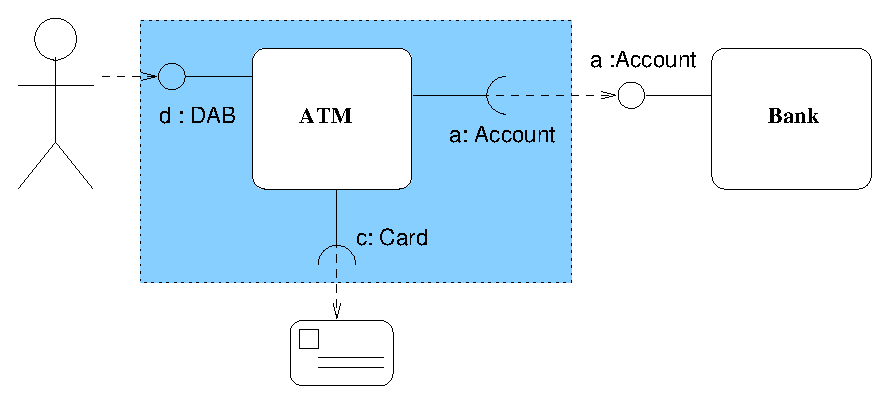
\includegraphics[width=.8\textwidth]{figures/fig-gab.eps}    
    \caption{Sch\'ema du guichet automatique}
    \label{fig-gab}
\end{figure}

Le composant ATM est le plus int\'eressant et c'est celui que nous
utiliserons par la suite dans l'illustration des techniques de
tests. Il offre une interface --- implicitement \texttt{unique} ---
permettant de r\'ealiser diverses op\'erations et requiert deux
ports : un port de type \texttt{Card} repr\'esentant le lien avec la
carte bancaire du client et un autre de type \texttt{Account}
repr\'esentant le lien avec la banque.

\begin{figure}[htbp]
\begin{lstlisting}
module Banque {
   exception error {};
   exception keep_card {};

  interface Card {...
  interface DAB { ...
  interface Account { ...

   component ATM {
      provides DAB d;
      uses Account a;
      uses Card    c;
      
   };
   
};
\end{lstlisting}
\centering
    
    \caption{Exemple de sp\'ecification \textsf{FIDL} : module Banque}
    \label{fig-exbanque}
\end{figure}

L'interface \texttt{Card} est d\'etaill\'ee dans la figure
\ref{fig-exifacecard}. Le num\'ero de compte est
stock\'e dans la carte et est donc le m\^eme pour toute la
dur\'ee d'une session, d'o\`u la d\'eclaration de
la variables $n$ englobant tous les \'echanges de messages. Le r\'esultat de
la m\'ethode \texttt{checkCode} est comme on peut s'y attendre
d\'ependant du code \og saisi\fg{} et est laiss\'e au soin de
l'implantation. Enfin la m\'ethode \texttt{failedCode} calcule le
nombre  de fois o\`u un code incorrect a \'et\'e saisi --- en examinant
toutes les r\'eponses \texttt{false} de la m\'ethode
\texttt{checkCode} --- et retourne cette valeur.

\begin{figure}[htbp]
\begin{lstlisting}
  interface Card {
    boolean checkCode(in long code); 
    long    failedCode();
    long    accountNo();

    /*** 
     header
       failed : Trace -> long
    FIDL
       n in (checkCode(_:_) +
        (f: f == failed(Trace) in failedCode(:f)) +
        accountNo(:n)))*

     body
       failed (~<-checkCode(False) : h) = (failed h) + 1;
       failed (_ : h) = failed h;
       failed [] = 0
    */
  };
\end{lstlisting}
    \centering
    
    \caption{Exemple de sp\'ecification FIDL : interface Card}
    \label{fig-exifacecard}
\end{figure}


L'interface \texttt{DAB}, figure \ref{fig-exifacedab}, d\'ecrit le comportement du guichet
automatique du point de vue du client. Le dialogue commence par
l'insertion de la carte, puis la saisie du code PIN et enfin les
diverse op\'erations. Cette interface sp\'ecifie en particulier que
les op\'erations ne sont accessibles que si le code saisi est correct
et si le nombre de saisies incorrectes est inf\'erieur \`a
3. L'exception \verb+keep_card+ peut-\^etre lev\'ee par chacune des
diff\'erentes m\'ethodes : elle signifie que la carte est
conserv\'ee par le guichet automatique et que plus aucune
op\'eration n'est possible avant de refaire une nouvelle
op\'eration \texttt{insert()} mod\'elisant le fait qu'une nouvelle
carte est introduite.

\begin{figure}[htbp]
    \centering
\begin{lstlisting}
   interface DAB {
     void    insert() raises (keep_card);
     boolean pinCode(in long code) raises (keep_card);
     void    withdrawCard () raises (keep_card);
     boolean withdrawal (in long amount) raises (keep_card);
     boolean transfer (in long amount,in long toAccountNo) raises (keep_card,error);
     long    balance () raises (keep_card);
     
     /*** FIDL
        (insert()
        ( 
          ((pinCode(_:false) + void) ( pinCode(_:false) + void)  pinCode(_:true)
            (
              withdrawal(_:_) +
              balance(:_) +
              -> transfer(_,_) (<-transfer(_) +  <-transfer<error>)) 
            )* withdrawCard() 
            ) 
            +
        ( 
           pinCode(_:false) pinCode(_:false) pinCode(_:false) 
           (
            (->withdrawal(_) <-withdrawal<keep_card>) +
            (->balance() <-balance<keep_card>) +
            (->transfer(_,_) <-transfer<keep_card>) +
            (->withdrawCard() <-withdrawCard<keep_card>)
           )
        ))*
       
     */
   };
\end{lstlisting}

    \caption{Exemple de sp\'ecification \textsf{FIDL} : interface DAB}
    \label{fig-exifacedab}
\end{figure}
 
Cet exemple relativement simple permet toutefois d'illustrer les
principaux concepts des sp\'ecifications \textsf{FIDL} dans le cas de
composants sans sp\'ecification propre. 

\subsection{Un syst\`eme de vote \'electronique}

Le deuxi\`eme exemple est celui d'un syst\`eme de vote
\'electronique. L'architecture du syst\`eme de vote est
repr\'esent\'ee sch\'ematiquement sur la  figure
\ref{fig-archivote} : il existe un certain nombre de composants
individuels de \emph{vote \'electronique} qui sont connect\'es \`a un
\emph{centre de vote} au travers d'une interface \texttt{Vote\_Center}
leur permettant de transmettre le vote --- un choix binaire ; et qui
par ailleurs peuvent recevoir un \'ev\'enement signifiant la
cl\^oture du scrutin --- type \texttt{Closure} --- et contenant le
r\'esultat du vote.

\begin{figure}[htbp]
    \centering
    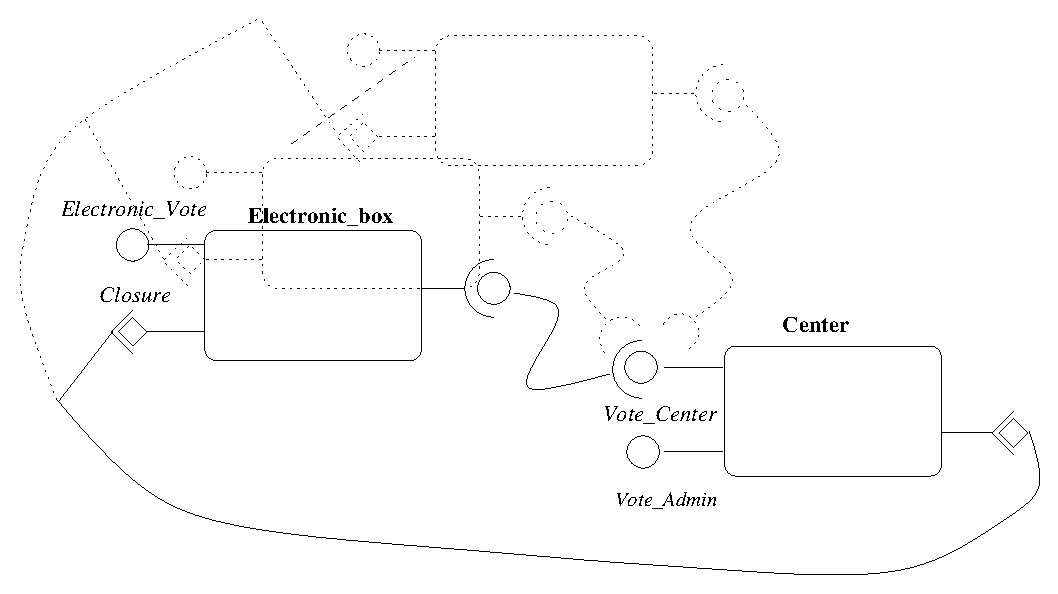
\includegraphics[width=.8\textwidth]{figures/exemple_vote.eps}
    \caption{Architecture du syst\`eme vote}
    \label{fig-archivote}
\end{figure}

Les types de donn\'ees utilis\'es sont d\'efinis dans le module
\texttt{Vote}, figure \ref{fig-exvote} : diverses exceptions, la
structure de l'\'ev\'enement de fermeture du scrutin et les
composants et interfaces. 

\begin{figure}[htbp]
    \centering
\begin{lstlisting}
module Vote { 
  exception too_late {};
  exception already_voted {};
  exception already_closed {};
  exception not_closed {};
  
  eventtype Closure {
    attribute long yes_number;
    attribute long no_number;
  };
  interface Electronic_Vote{ ...
  interface Vote_Center { ...
  interface Vote_Admin { ...
  component Center { ...
  component Electronic_Box { ...

};  
\end{lstlisting}
        \caption{Exemple 2 : module Vote}
    \label{fig-exvote}
\end{figure}

L'interface \texttt{Electronic\_Vote} (figure \ref{fig-exifacevote}) repr\'esente l'interaction
entre chaque bo\^{\i}te individuelle de vote et l'utilisateur. Son
fonctionnement est simple : elle permet \`a l'utilisateur de voter
une et une seule fois, et refuse pendant un certain temps de fournir
le r\'esultat du scrutin, puis fournit toujours le m\^eme r\'esultat. On notera l'utilisation
de l'op\'erateur  \verb+||+ qui permet d'entrelacer
arbitrairement les appels aux diff\'erentes m\'ethodes de
l'interface --- tout en respectant les r\`egles de formation correcte
des \'echanges de messages, et le fait que rien n'est dit dans l'interface quant au
moment o\`u le r\'esultat est disponible.

\begin{figure}[htbp]
    \centering
\begin{lstlisting}
  interface Electronic_Vote{ 
    boolean vote (in boolean choice);
    boolean results(out long yes,out long no);
    
    /*** FIDL
       (c in vote(c:true) + void) (c in vote(c : false) )*
     ||(results(_,_:false)*(x,y in results(x,y:true)*)) 
    */
  };
\end{lstlisting}
        \caption{Exemple 2 : interface de vote \'electronique}
    \label{fig-exifacevote}
\end{figure}
  
L'interface suivante, \texttt{Vote\_Center}, est fournie par le centre
de vote pour r\'ecup\'erer les diff\'erents votes. Son
fonctionnement est sym\'etrique de celui de l'interface
pr\'ec\'edente : elle permet de voter une et une seule fois, et
\'eventuellement elle interdit le vote si celui-ci survient trop
tard. L'interface d'administration, enfin, permet de clore le
scrutin une et une seule fois (voir figure \ref{fig-exifacecenter}).

\begin{figure}[htbp]
    \centering
\begin{lstlisting}
  interface Vote_Center {
    void vote (in boolean choice) raises (too_late,already_voted);
    
        /*** FIDL
           (x  in vote(x)) (x  in ->vote(x) <-vote<already_voted> + void)*
           (x in ->vote(x) <-vote<too_late> )* 
        */
  };
    
  interface Vote_Admin {
    void close() raises (already_closed);
    
      /*** FIDL
        close() (->close() <-close<already_closed>)*
      */
  };
\end{lstlisting}
        \caption{Exemple 2 : interfaces centre de vote \& administration}
    \label{fig-exifacecenter}
\end{figure}


Les sp\'ecifications des composants sont ici bien plus
int\'eressantes car elles permettent de \emph{mettre en musique} le
comportement des interfaces et de pr\'eciser, par exemple,
l'ordonnancemnt des diff\'erents \'ev\'enements. Le composant \texttt{Center}
est d\'etaill\'e dans la figure \ref{fig-excenter} : c'est lui qui
calcule le r\'esultat du vote en fonction des votes re\c{c}us et
effectivement pris en compte (fonction \texttt{result}) et qui
pr\'ecise \`a l'aide de l'op\'erateur de composition \texttt{and} comment
la cl\^oture du vote interagit avec les votes. Le choix fait dans
cette sp\'ecification est que tout vote survenant apr\'es un
\emph{appel} de \texttt{close()} n'est plus pris en compte, un autre
choix possible e\^ut \'et\'e de  prendre quand m\'eme en compte
ces votes. 
 
\begin{figure}[htbp]
    \centering
\begin{lstlisting}
  component Center { 
    
    provides Vote_Center v;
    provides Vote_Admin a;
    publishes Closure c;
    /***
        header
        result : Trace, boolean -> long

        FIDL
           a->close() (x : x == result(Trace,true), 
                       y : y == result(Trace,false) in c[x,y])
           a<-close() a.close<already_closed>*
         and 
           (v.vote(_) (x in v->vote(x) v<-vote<already_voted>)* + void)
           (
               (a.close() (a.close<already_closed>* || 
                           (v->vote(_)v<-vote<too_late>)*)) 
               +            
               (a->close() || v->vote(_)) 
               (v<-vote<too_late> (v->vote(_)v<-vote<too_late>)* ||
                a<-close() (a->close() a<-close<already_closed>)*)
           )
            
           body
           result [] _  =  0;
           result (~v->vote(x) : ~v<-vote() : h) y = if x == y 
                                                     then (result h x) + 1 
                                                     else (result h x);
        */
  };
\end{lstlisting}
        \caption{Exemple 2 : composant centre de vote}
    \label{fig-excenter}
\end{figure}

Le composant \texttt{Electronic\_Box} enfin (figure
\ref{fig-exevote}), permet de pr\'eciser le comportement de
l'interface de vote \'electronique en relation avec l'\'ev\'enement
de notification de fermeture du scrutin. 

\begin{figure}[htbp]
    \centering
\begin{lstlisting}
  component Electronic_Box {
    provides Electronic_Vote e;
    uses Vote_Center v;
    consumes Closure c;
        
        /*** FIDL
               (x  in e->vote(x) ( v.vote(x) e<-vote(:true) + 
                                   v->vote(x) v<-vote<too_late> e<-vote(:false)
                                 )
               ) e.vote(_:false)*
           and 
               e.results(_,_:false)
               (x,y in (c[x,y] + e->results() c[x,y] c[_,_]*
               e<-results(x,y:true)) (e.results(x,y:true)* || c[_,_]*))
        */
  };
\end{lstlisting}
        \caption{Exemple 2 : composant bo\^{\i}te individuelle de
           vote }
    \label{fig-exevote}
\end{figure}

On voit donc bien que c'est la sp\'ecification des composants qui
donne la s\'emantique du syst\`eme de vote et qui a pour fonction
d'assurer simultan\'ement l'unicit\'e des votes r\'ealis\'es au
moyen de chacune des bo\^{\i}tes \'electroniques, ce qui est
sp\'ecifi\'e par l'interface de vote \'electronique ; et par
ailleurs de garantir que tous les votes effectu\'es avant la
cl\^oture du scrutin soient pris en compte dans le d\'ecompte final
des voix qui d\'epend justement de la cl\^oture du scrutin. 
On verra  au chapitre consacr\'e \`a la composition
comment \`a partir de ces sp\'ecifications on peut esp\'erer
v\'erifier certaines propri\'et\'es du syst\`eme.



% $Log : fidl.tex,v $
% Revision 1.25  2004/10/18 09:16:33  bailly
% suppression etat art g\'en\'eral
% ajout etat art par partie (composants et test)
%
% Revision 1.24  2004/06/08 15:38:53  bailly
% *** empty log message ***
%
% Revision 1.23  2004/06/02 15:32:44  bailly
% merging
%
% Revision 1.22  2004/06/02 07:23:07  bailly
% promotion en chapitre des sections modeles et automates
%
% Revision 1.21  2004/03/29 09:26:14  bailly
% Corrections ISA suite
%
% Revision 1.20  2004/03/26 16:37:36  bailly
% *** empty log message ***
%
% Revision 1.17  2004/03/01 15:01:39  bailly
% Corrections FIDL
%
% Revision 1.16  2004/02/25 12:39:16  bailly
% Fin correction ISa sur langage FIDL
% Modification calcul ens traces de composite, syst\`eme, agencement
% Modification calcul environnement
%
% Revision 1.15  2004/02/24 08:35:55  bailly
% *** empty log message ***
%
% Revision 1.14  2004/02/24 08:26:37  bailly
% *** empty log message ***
%

%%% Local Variables: 
%%% mode: latex
%%% TeX-master: "these"
%%% End: 
